\documentclass[reprint,amsmath,amssymb,aps,showpacs,onecolumn,superscriptaddress,prb]{revtex4-1}

\usepackage{graphicx}
\usepackage{bm}
\usepackage{epsfig}
\usepackage{amssymb}
\usepackage{amsfonts}
\usepackage{braket}
\usepackage{color}
\usepackage{epstopdf}
\epstopdfsetup{update}
\usepackage{hyperref}
\usepackage{float}
\restylefloat{table}
\usepackage{bibentry}
\usepackage{multirow}
\usepackage[caption=false]{subfig}
\newcommand{\ba}{\begin{eqnarray}}
\newcommand{\ea}{\end{eqnarray}}
\newcommand{\bd}{\begin{displaymath}}
\renewcommand{\v}[1]{{\bf #1}}
\newcommand{\nn}{\nonumber \\}


\begin{document}
\title{Supplementary Materials for ``Machine-learning Skyrmions''}

\author{Vinit Kumar Singh}
\email[Electronic address:$~~$]{vinitsingh911@gmail.com}
\affiliation{Department of Physics, Indian Institute of Technology, Kharagpur 732102, India}
\author{Jung Hoon Han}
\email[Electronic address:$~~$]{hanjh@skku.edu}
\affiliation{Department of Physics, Sungkyunkwan University, Suwon 16419, Korea}
\date{\today}
%\begin{abstract}
%We present several figures as supplementary information to the main paper.
%\end{abstract}
\maketitle
\begin{widetext}

\section{PCA and correlation function}

Several leading eigen-images obtained from diagonalizing the correlation matrix of each phase are shown in Fig. \ref{fig:SMfig1}. The correlation function $[\bf C]_{i\alpha, j\beta}$ can be summed up as

\ba C_{\v r}^{\alpha\beta} = \sum_i [\bf C]_{i\alpha, i+\v r \beta} .\ea
Such correlation function $C_{\v r}$ is shown for diagonal ($\alpha\beta=xx$) and off-diagonal ($\alpha\beta=xy$) spin correlations in Fig. \ref{fig:SMfig2}.

\begin{figure}[ht]
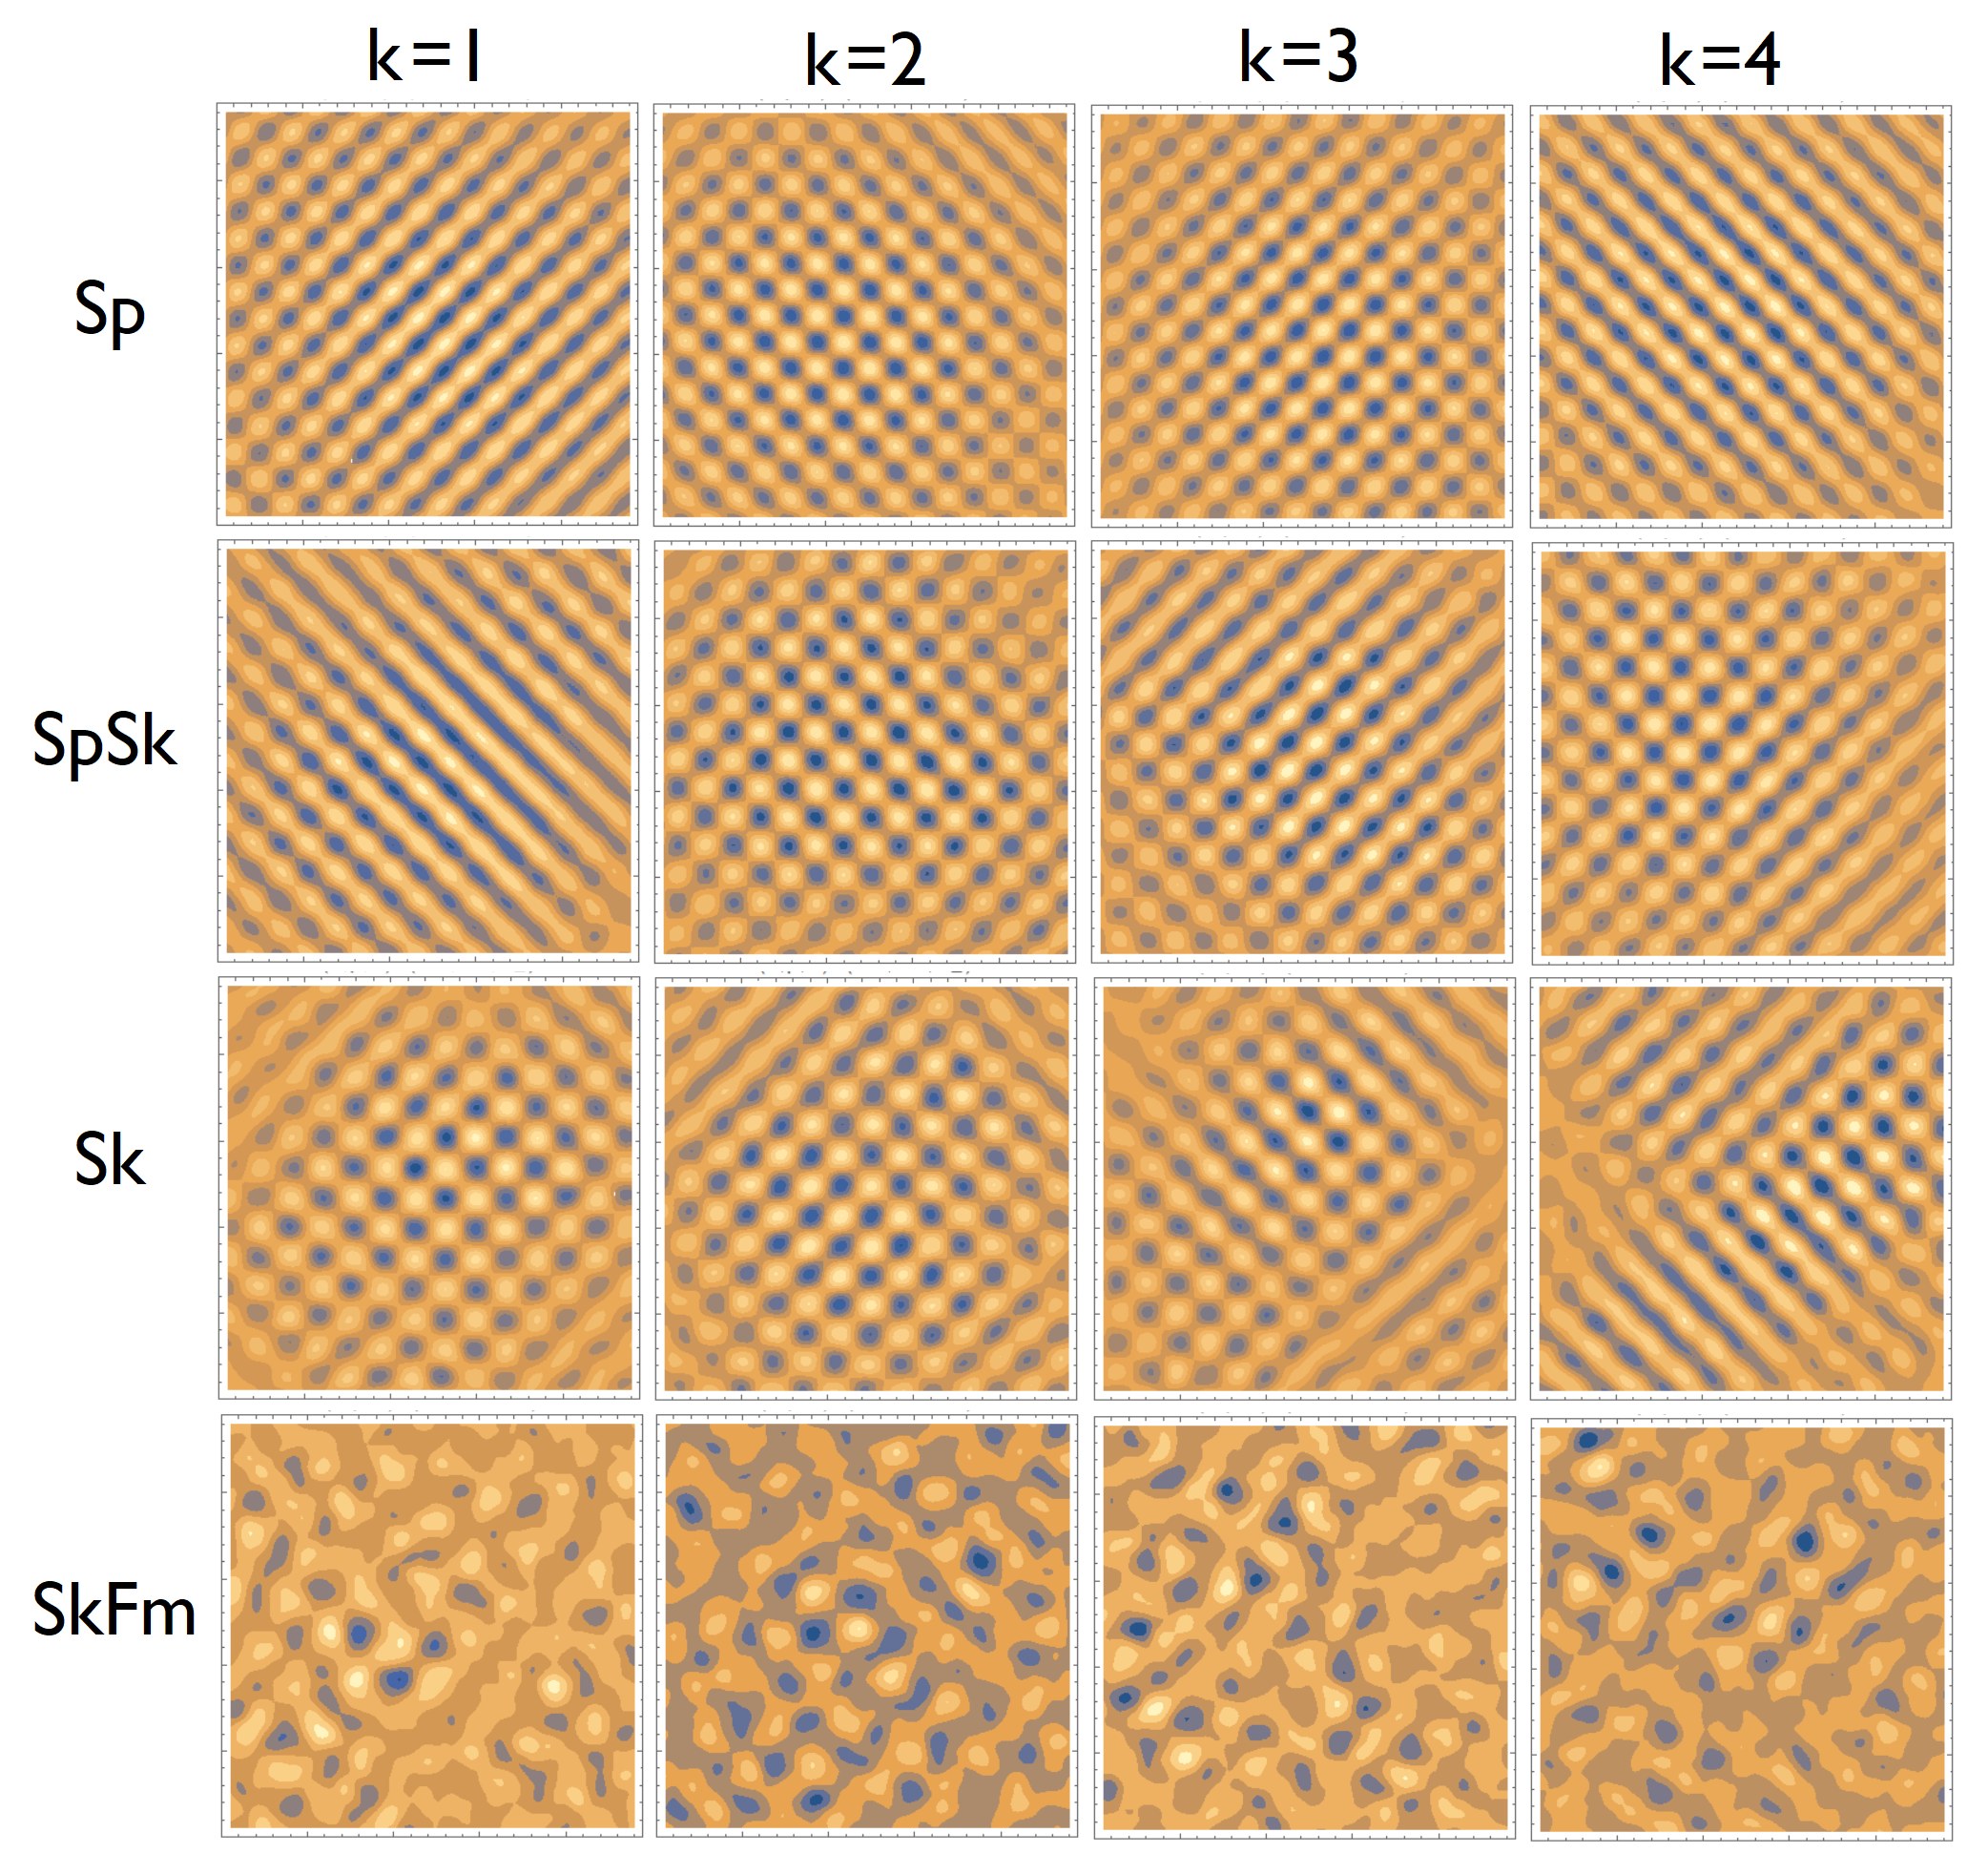
\includegraphics[scale=0.35]{SMfig1.png}
\caption{The first four leading eigen-images of the correlation matrix from Sp, SpSk, Sk, and SkFm phases.}\label{fig:SM1}
\end{figure}

\begin{figure}[ht]
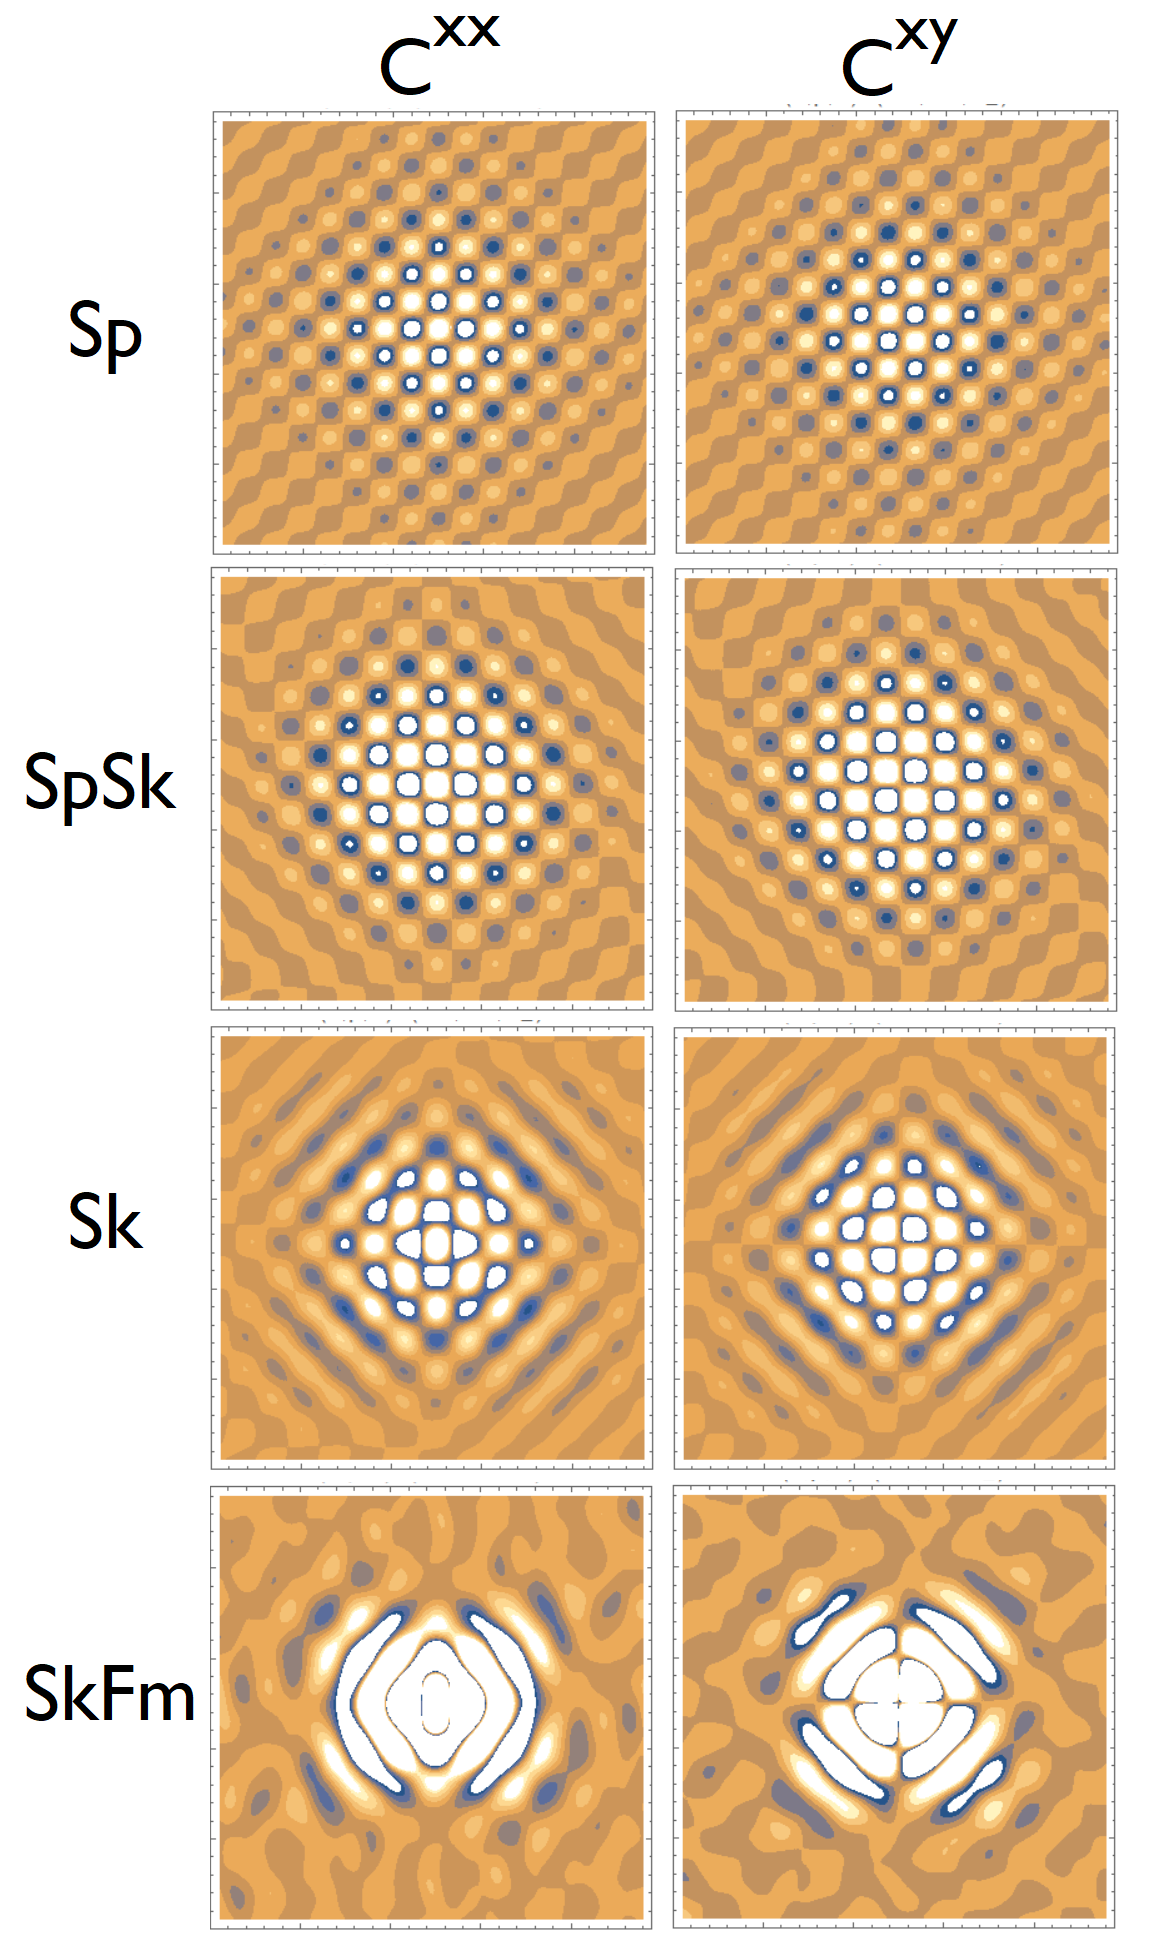
\includegraphics[scale=0.4]{SMfig2.png}
\caption{Spin-spin correlation function for diagonal ($xx$) and off-diagonal ($xy$) spin correlations.}\label{fig:SM1}
\end{figure}

\section{Machine learning of phases}

As an initial application of ML ideas to the HDMZ model, Our training set was generated by the Monte Carlo (MC) method with $D/J=\sqrt{6}$, corresponding to the spiral period $\lambda=6$. The inter-skyrmion distance in the skyrmion phase is also of the same order. The average spin chirality $\chi$ over the $(T,B)$ plane is presented in Fig. 2(a). Judging from the lack of significant spin chirality, the $B\in [0, 1.2]$ region over the temperature $T\in [0.03, 0.25]$ (box 1 in the chirality map, Fig. 2) can be said to belong to the spiral phase. Likewise, one can say with confidence that $B\in [3.4, 4.2]$ over $T\in [0.03, 0.25]$ belongs to the ferromagnetic phase (box 5 in Fig. 2). Here $T=0.03$ is the lowest temperature reached in our MC calculation. The robust skyrmion phase can be found at $B\in[1.8, 2.6]$ (box 3). For each $B$, the temperature interval $T \in [0.03, 2.0]$ was divided into 40 steps using adaptive scheduling, {\it i.e.} exponentially decaying step size with a decay rate of 0.1. That gave us a total of 20 steps from the interval $T \in [0.03, 0.25]$, and with each step we drew 100 MC configurations. Finally, 17 different magnetic field values were selected, for a total of $20 \times 100\times 17 = 34,000$ training configurations. Training with the much larger training set of 330,000 configurations did not change the final results.

The  ML  architecture used  for  the  training  involved an  initial CNN  layer  of  $6\times 6$  filter  size  (since  the skyrmion  diameter  and  period  of  spirals  are  both  6)  and a second CNN layer with $3\times3$ filter size both accompanied  with  Max  Pool  filters,  followed  by  flatten and two  dense neural  network  layers  containing  512,  1024  neurons  respectively, which then led to the output layer. Batch normalization and dropout regularization are applied to outputs from each layer. The schematic diagram of the architecture can be found in the Supplementary Material (SM). The final outcome was then compared to one of three values, 0, 1, 2, corresponding to spiral, skyrmion, and ferromagnetic phases, respectively. The training data was initially prepared in terms of spin angles $(\theta_i , \phi_i )$, which gave far poorer results than if the data was prepared in terms of the magnetization $\v n_i = (\sin \theta_i \cos \phi_i, \sin \theta_i, \sin \phi_i, \cos\theta_i)$. All the ML analysis presented in this paper is thus based on the magnetization inputs. The architecture consisting purely of the deep neural network layer did not work as well as the one we used, involving the CNN filter layer as well. Further minute changes in the architecture had little impact on the overall quality of final results. After training, the validation procedure gave nearly 100\% correct values for the phase labels. This is not surprising given the fact that validation sets also came from deep inside one of the three phases.

For testing purpose we generate a new batch of MC configurations at $T\in [0.03, 0.25]$ and $B\in [1.2, 1.8]$ (box 2 in Fig. 2), which admittedly belongs to the SpSk mixed phase, and another batch at $T\in [0.03, 0.25]$ and $B\in [2.6,3.4]$ (box 4 in Fig. 2) belonging to the SkFm mixed phase. At each $(T,B)$, 100 configurations were generated and fed to the machine for prediction. The answers given by the machine are then averaged over and shown as probabilities for spiral, skymion, and ferromagnetic phase, in Fig. 2 (b) and (c). Since the temperature range was quite small and the variations in the configurations were minor, the answers were averaged over all the 20 temperature steps in the interval $T\in [0.03, 0.25]$ as well. Despite the fact that each data point in Fig. 2(b) and (c) represents an average over $100\times 20 = 2,000$ configurations, and that extremely fine steps in magnetic field $\Delta B= 0.01$ was used, the final results are far from being smooth. The ML program trained on the three distinct phases of the skyrmion model, on the other hand, fails quite dramatically to make continuously varying predictions for its mixed phases. Since the temperature range was quite small and the variations in the configurations were minor, the answers were averaged over all the 20 temperature steps in the interval $T\in [0.03, 0.25]$ as well. Despite the fact that each data point in Fig. 2(b) and (c) represents an average over $100\times 20 = 2,000$ configurations, and that extremely fine steps in magnetic field $\Delta B= 0.01$ was used, the final results are far from being smooth.


Supplementary figure \ref{fig:SM1} shows the machine-learning architecture we used to train various features of the skyrmion model. The input size is $(L,L,3)$ for $L\times L$ lattice since we are using three components of the magnetization vector to represent the data at each site.  The skyrmion diameter and period of spirals are both 6 for the parameter choice $D/J=\sqrt{6}$. To have a faithful representation of this periodicity in the lattice over the hidden layers, an initial CNN layer with 16 filters, each of size 6$\times$6, was used, altering the input size to $(L-5, L-5, 16)$. The first CNN layer was followed by the Max Pool layer of 2$\times$2 filter size, which reduces the input size to $([ ( L-5 ) /2 ] , [ (L - 5 ) /2 ] , 16)$. It is then followed by a second CNN layer with 32 (3$\times$3) filters, changing the input size to $([ ( L-5 ) /2 ] -2 , [ ( L-5 ) /2 ] -2 , 32)$.  Batch Normalization and Dropout Regularization accompanied both CNN layers. After applying the second Max Pooling to reduce the size to $([([(L-5)/2]-2)/2], [([(L-5)/2]-2)/2], 32)$, the input data was flattened to $([([(L-5)/2]-2)/2]\times [([(L-5)/2]-2)/2] \times 32, 1)$. Square bracket represents the ceiling function. This was then fed through two Dense Neural Network (DNN) layers containing 512, 1024 neurons respectively, which then led to the output layer. Batch normalization and Dropout Regularization are applied to outputs from each DNN layer. Leaky ReLu was employed as the activation function with $\alpha=0.1$, except for the output layer where a sigmoid function was used. Adam optimizer and Learning Rate Scheduler were applied to enhance the training speed.

In the label prediction, one-hot encoded labels were used to represent different phases: (1,0,0) for spiral, (0,1,0) for skyrmion and (0,0,1) for ferromagnetic.  Binary cross entropy was used as the Loss function. In the feature prediction,  values of $(\chi,  m, B, T)$ were rescaled to the $(0,1)$ range and mean-squared error was used as the loss function.

\begin{figure}[ht]
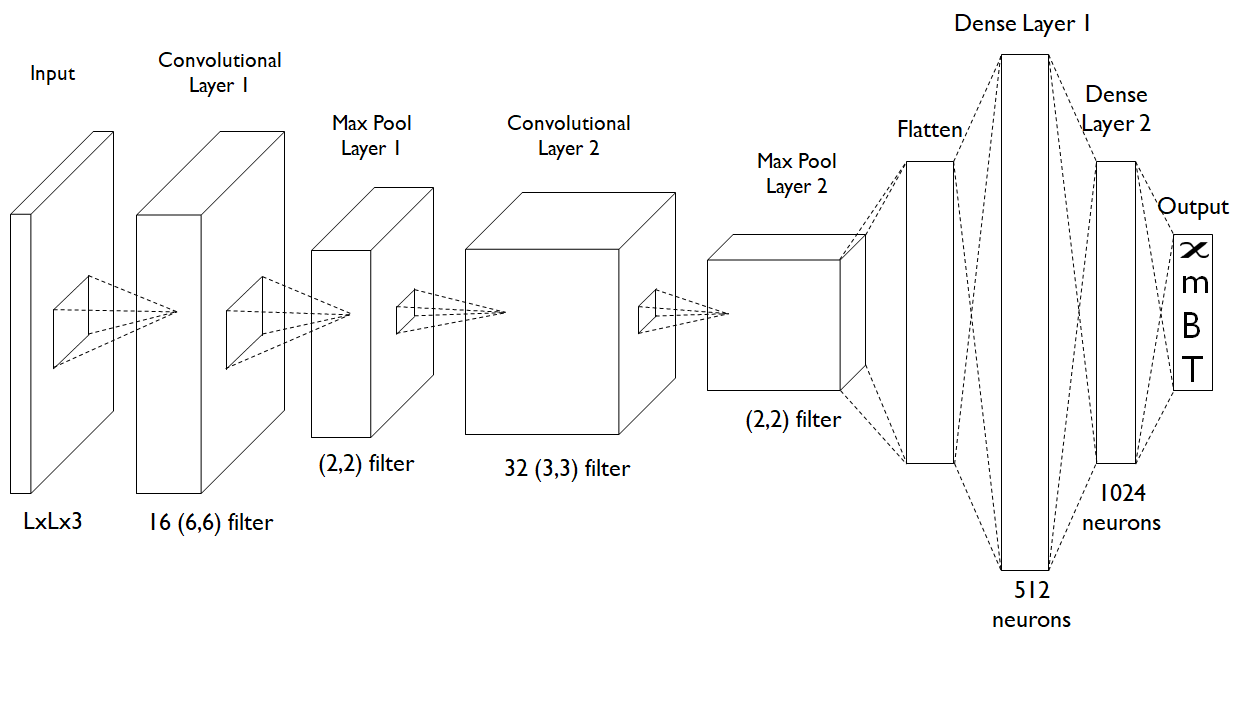
\includegraphics[scale=0.5]{SMfig3.png}
\caption{Schematic diagram of the ML architecture used in the paper.}\label{fig:SM1}
\end{figure}

\section{Machine learning for various Hamiltonians}

Supplementary figure \ref{fig:SM2} gives a collection of $(\chi, m, B, T)$ predictions at various values of $(K,p)$ which are not shown in the main text.

\begin{figure}[ht]
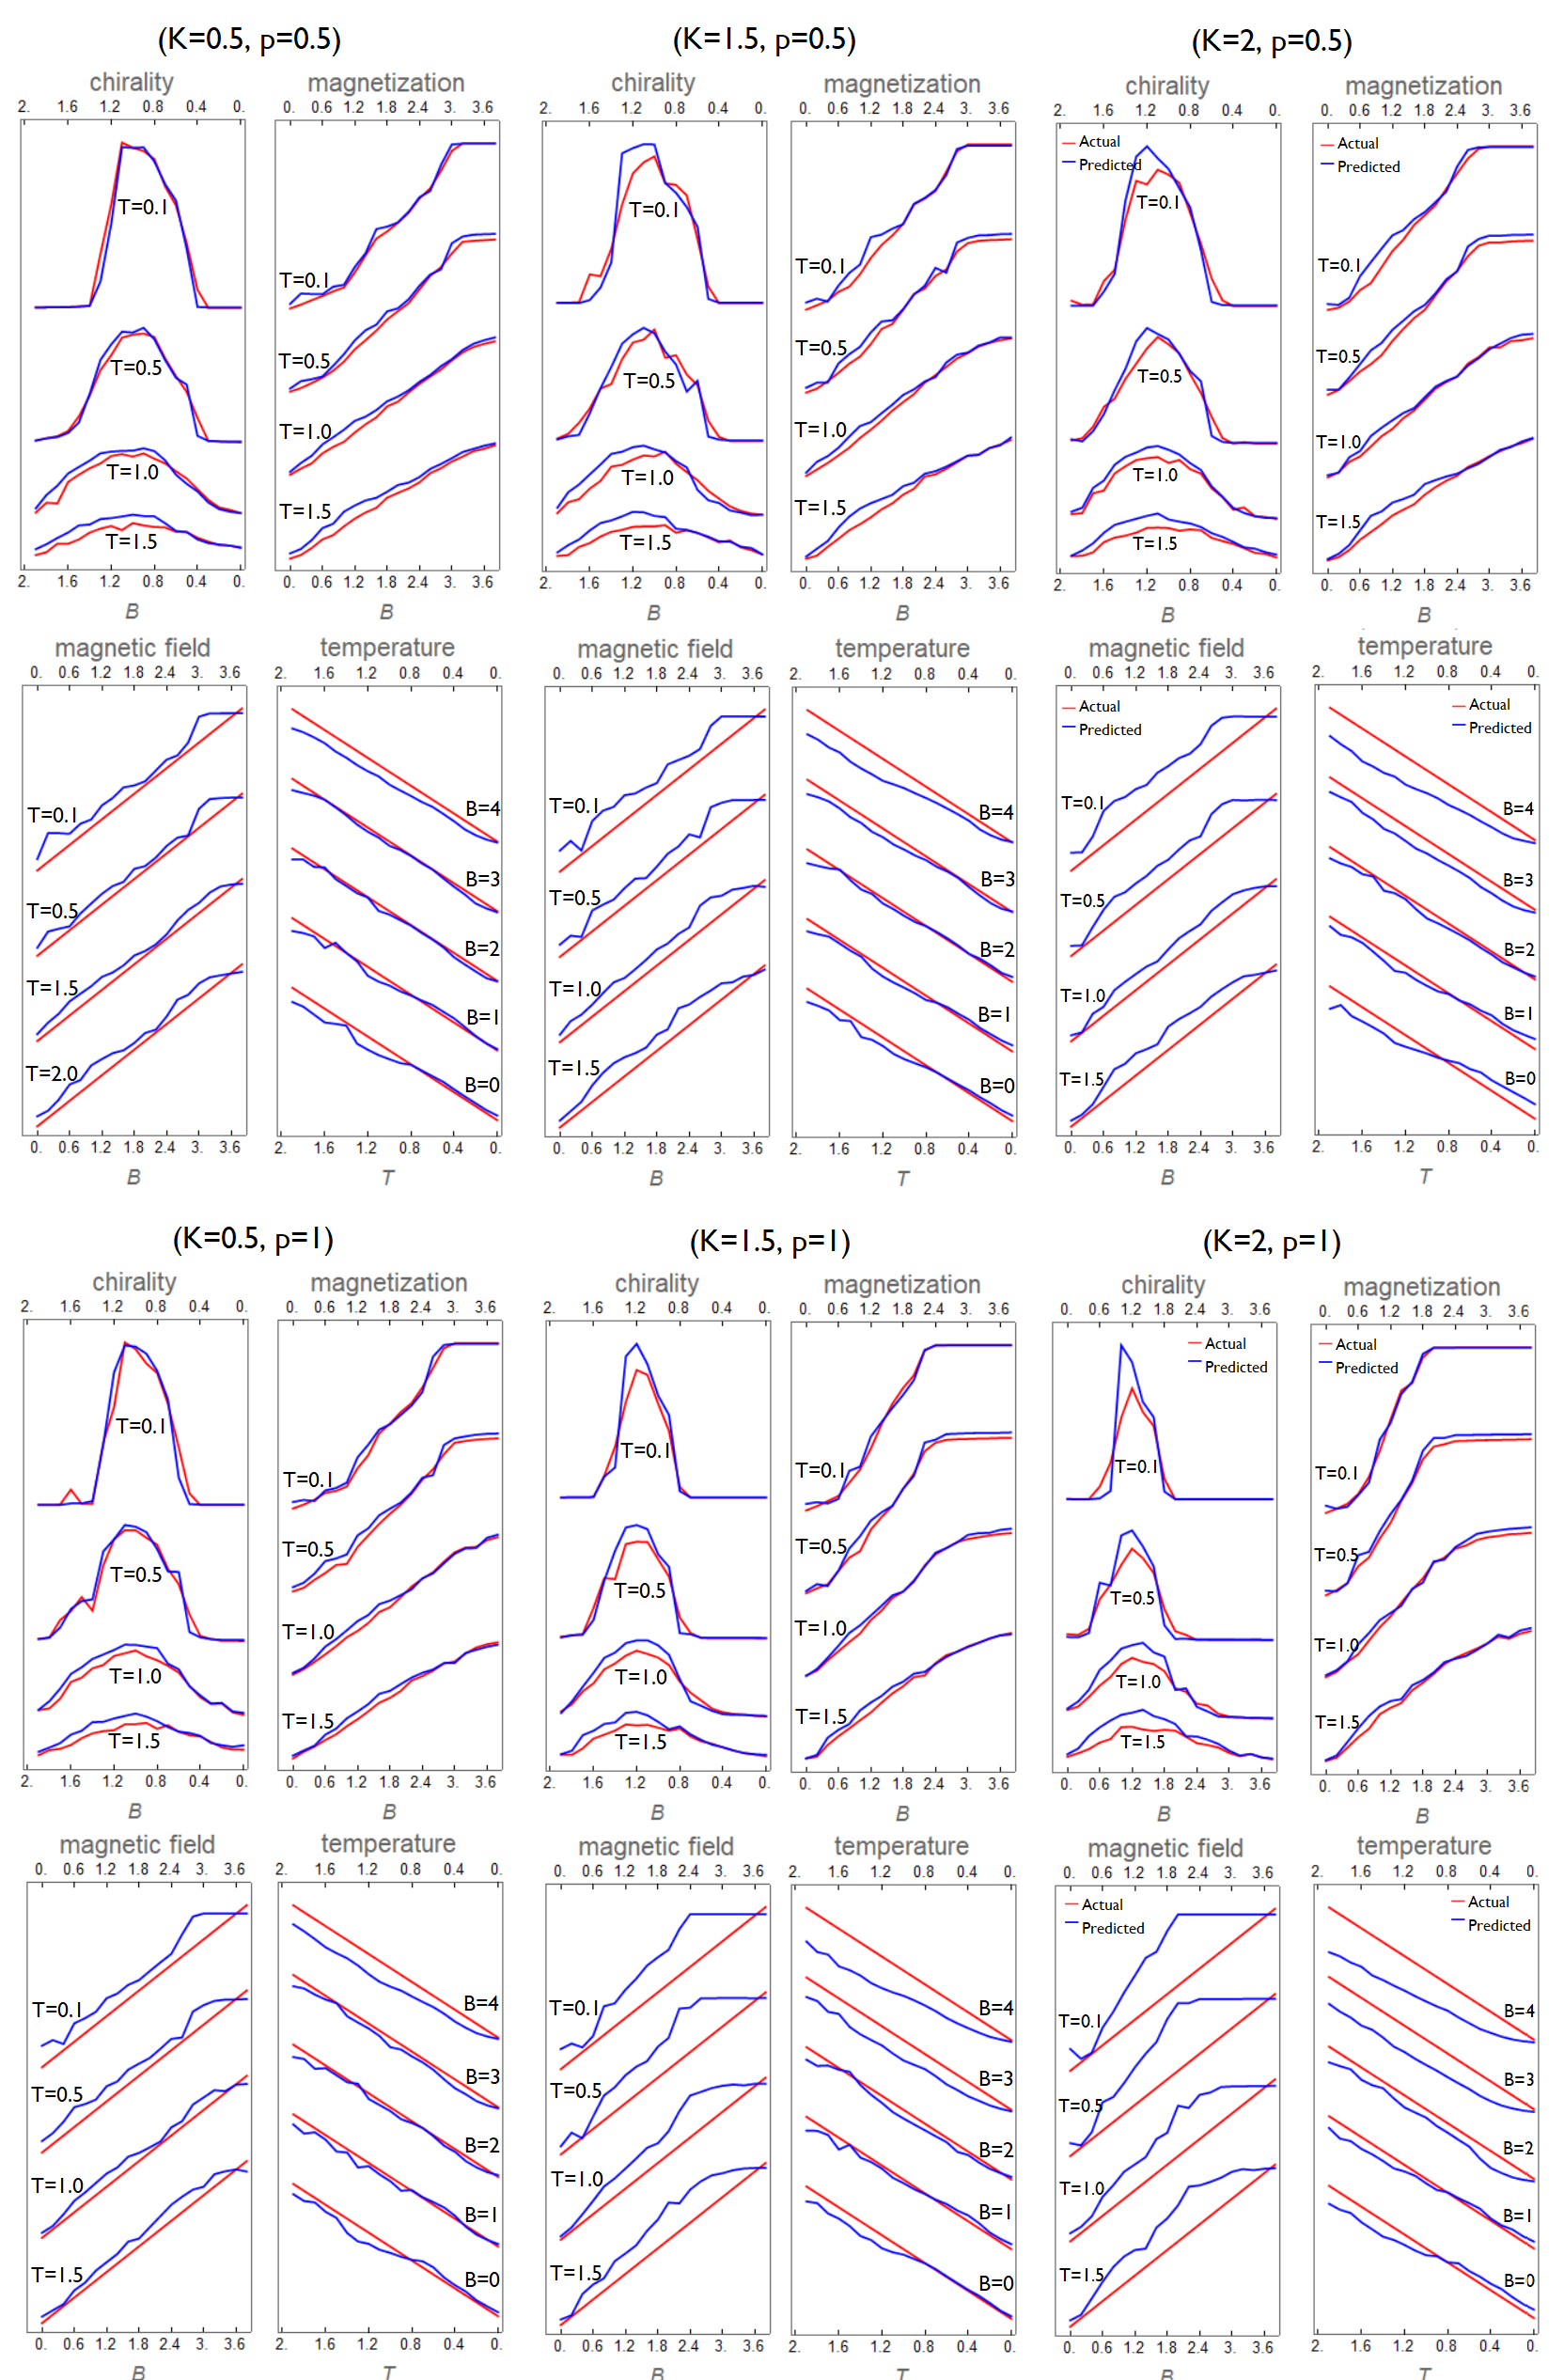
\includegraphics[scale=0.45]{SMfig4.png}
\caption{Comparison of actual and machine-predicted values of $(\chi, m, B, T)$ for several values of $(K,p)$.}\label{fig:SM2}
\end{figure}
\end{widetext}


\begin{thebibliography}{99}
\end{thebibliography}

\end{document}
